%
%% Exercise 3
%
\subsection{Question 1}
We assume that the probability of each passenger showing up is 0.95 (since probability of not showing up is 0.05), and that the event of a passenger showing up is independent (which is the case according to the description).
Which implies $P[passenger showin gup] = 0.95$, from which we can calculate

\begin{align}
\left( \frac{95}{100} \right)^{100} = 0.00592... \approx 0.006	
\end{align}
So for 6 out of 1000 flights there might show up too many passengers, so the plane won't have enough seats left for all passengers in those cases.

\subsection{Question 2}
We have given the following Events:
\begin{enumerate}
	\item 95\% of passengers showing up out of 10000, where each passenger shows up with the probability $p$
	\item 100 passengers show up each with the probability of $p$ (everybody shows up)
\end{enumerate}

From those 2 Events we get the probability that 9500 of 10000 persons getting on their plane and all 100 passengers arriving to one given airplane (overbooking).
With this information we use the hoeffding bound for the probability of 9500 arriving to a plane.
When this bound is found we then can multiply it by the probability that a plane gets overbooked ($p^{100}$).
Then I can solve for $p$ and find the bound.
 
\begin{align}
	&\Prob \left( \sum_{i=1}^{10000} X_{i} \geq 9500 \right) \\
	= &\Prob \left( \sum_{i=1}^{10000} X_{i} - 10000\cdot p \geq 9500 - 10000\cdot p \right)  \\
	\leq &e^{-2(10000(0.95-p))^2 / \sum_{i=1}^{10000}(b_{i} - a_{i})^{2}} \\
	=& \leq e^{-2(10000(0.95-p))^2 / \sum_{i=1}^{10000}(0 - 1)^{2}} \\
	=&  \leq e^{-2(10000(0.95-p))^2 / \sum_{i=1}^{10000}1} \\
	=&  \leq e^{-2(10000(0.95-p))^2 / 10000}
\intertext{Now using the expression for the probability (bound) of all people arriving to the plane $p^{100}$ the probability can be bound:}
	&p^{100}\cdot e^{-2(10000(0.95-p))^2 / \sum_{i=1}^{10000}1}  = 0.006797
\end{align}
 
When we solve the equation numerically we will find $p=0.9526$.
 The figure below (figure \ref{fig:ex3} shows the corresponding bound given probability $p$.

\begin{figure}[!htb]
	\center
	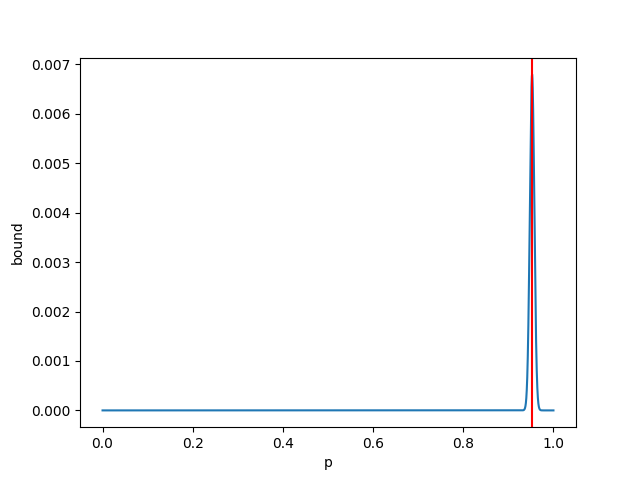
\includegraphics[width=\textwidth]{code/ex3}
	\caption{showing the bound to the corresponding probability, while the red line is the worst case p}
	\label{fig:ex3}
\end{figure}